\documentclass[style=upen, size=14pt]{powerdot}
\usepackage{natbib}
\usepackage{mathtools}
\definecolor{arany}{RGB}{255,242,0}
\hypersetup{backref=page}
\hypersetup{
    colorlinks=true,
    linkcolor=cyan,
    citecolor=cyan,
    filecolor=magenta,      
    urlcolor=cyan}
% \pdsetup{trans=Split}
\usepackage{graphicx}
\usepackage{amsmath}
\DeclareMathOperator*{\argmax}{argmax}
\DeclareMathOperator*{\argmin}{argmin}
\DeclareMathOperator*{\softmax}{softmax}
\DeclareMathOperator{\sign}{sign}
\usepackage{amssymb}
\usepackage{stmaryrd}
\usepackage[latin2]{inputenc}
%\usepackage[magyar]{babel}
%\usepackage{euler}
\usepackage{tikz}
\usetikzlibrary{matrix}
%\usepackage{tikz-qtree}
%\usepackage{tikz-dependency}
%\usepackage{linguex}
\usepackage{amsthm}
\usepackage{amsmath}
%\tikzset{every tree node/.style={align=center,anchor=north}}
%\usepackage{tabularx}
%\usepackage{threeparttable}
%\usepackage{color}
%\selectlanguage{english}
%\frenchspacing
\usepackage{algpseudocode}
\usepackage{algorithm}
\newcommand\varlist{,\makebox[1em][c]{.\hfil.\hfil.},}
\newcommand{\nd}{\noindent}
\newcommand{\Val}{\mathop{\mathit{Val}}}
\newcommand{\gold}{\color{arany}}
%\usepackage{tikz}
%\usepackage{tikz-qtree}
%\newcommand{\qed}{\hfill\mbox{\raggedright \rule{.1in}{.1in}}}
\def\es{\mathbin\land}
\theoremstyle{definition}
\newtheorem*{definition}{Definition}
\newtheorem{axioma}{Axiom}
\newtheorem{tetel}{Theorem}
\newtheorem{prop}{Proposition}
\newtheorem{lemma}{Lemma}
\begin{document}

\title{Natural Language Processing\\~~\\Lecture 8\\Static neural word embeddings}
% \author{}

\date{2021}
\maketitle

\begin{slide}[toc=Vectors and NNs]{Word vectors and neural networks}
  The success of LSI and LSA showed that distribution based vector
  representations of words can be very useful for NLP tasks in general. In the
  case of neural network NLP models, continuous, dense word representations have
  been especially important, because they
  \begin{itemize} 
  \item can be used as informative and economic representations instead of
    simply one-hot encoding words;
  \item can help decreasing the number of model parameters;
  \item can be learned by neural networks from text corpora in a self-supervised
    manner.
  \end{itemize}
\end{slide}

\begin{slide}[toc=]{Word vectors and neural networks cont.}
  One of the first instances of word vectors learnt by a neural network can be
  found in the neural language model of \cite{bengio2003neural}:
  \begin{center}
  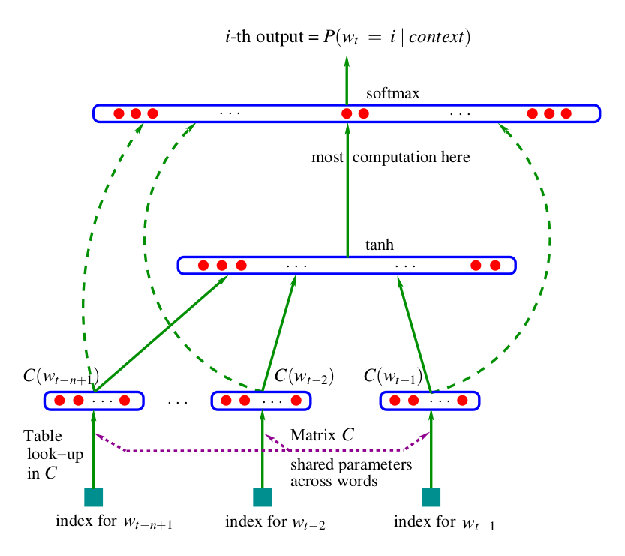
\includegraphics[width=0.6\textwidth]{figures/neural_lm.eps}
  \end{center}
\end{slide}

\begin{slide}[toc=]{Word vectors and neural networks cont.}
  $C$ is an embedding layer mapping word vocabulary indexes to vectors of real
  numbers:
  $$
  C: [0, |V|)  \rightarrow \mathbb R^d.
  $$
  The $d$ dimensionality of (static) word embeddings is typically within the
  50--600 range.

  Technically, embedding layers can be implemented in several ways, e.g., as a
  dense layer with one-hot encoded word indexes as input (in this case the word
  vectors are represented as the weight matrix of the layer), or as a look-up
  table represented as an array etc.
\end{slide}

\begin{slide}[toc=]{Word vectors and neural networks cont.}
  Important lessons regarding the embedding layer in \cite{bengio2003neural}:
  \begin{itemize}
  \item The model using the end-to-end trained word embedding layer performed
    better than traditional \emph{n}-gram based language models.
  \item Using the first principal components of the word co-occurrence frequency
    matrix as word feature vectors instead of the trained embeddings did not
    have the same performance benefits.
  \item Learning word embeddings with neural nets is a viable way of scaling up
    the training corpus. 
  \end{itemize}
\end{slide}

\section{Word2vec}

\begin{slide}[toc=Novelties]{Distinguishing features}
  Word2vec, introduced by \cite{mikolov2013efficient}, is also a neural network
  family learning useful distributed representations of words from a corpus, but
  with several novel features:
  \begin{itemize}
  \item It is a dedicated architecture: \emph{representation learning} is its
    sole goal.
  \item It is based on a new type of corpus-based, self-supervised predictive
    task.
  \item The architecture is kept intentionally very simple to make it possible
    to train on huge corpora with large vocabularies.
  \end{itemize}
\end{slide}

\begin{slide}[toc=Skipgrams]{Skipgrams}
  Word2vec is based on \emph{skipgrams}, which are a generalization of
  $n$-grams: while an $n$-gram is a \emph{continuos}, $n$-long subsequence of a
  text, skipgrams can contain a certain amount of ``jumps'': If the base
  sequence is $\langle w_1\varlist w_N\rangle$ then the set of $n$-long
  skipgrams with at most $k$ total distance is
  $$
  \{\langle w_{i_1} \varlist w_{i_n}\rangle~|~ i_1\varlist i_n\in[1, N],
  \sum_{j=2}^n i_j-i_{j-1} \leq k \}.
  $$
  There can be additional restrictions, e.g. on the number and length of
  individual skips.
\end{slide}

\begin{slide}[toc=Tasks]{Word2vec tasks}
  The Word2vec task is specifically based on skipgrams of length $2c$ with a
  single one-word skip at the center. There are two task-variants with
  associated model architectures:
  \begin{itemize}
  \item \emph{\gold CBOW} (Continuous Bag of Words): predict the missing word at
    the center of a skipgram. 
  \item \emph{\gold SkipGram}: predict the elements of the skipgram given the
    missing/skipped word. In contrast to the CBOW task, where each skipgram
    corresponds to exactly one classification example, the SkipGram task
    produces a $\langle$word-in-the-center word-from-the-skipgram$\rangle$
    example for each $2c$ word of a skipgram.
  \end{itemize} 
\end{slide}

\begin{slide}[toc=]{Word2vec tasks cont.}
  A simple illustration of the two tasks:
  \begin{center}
    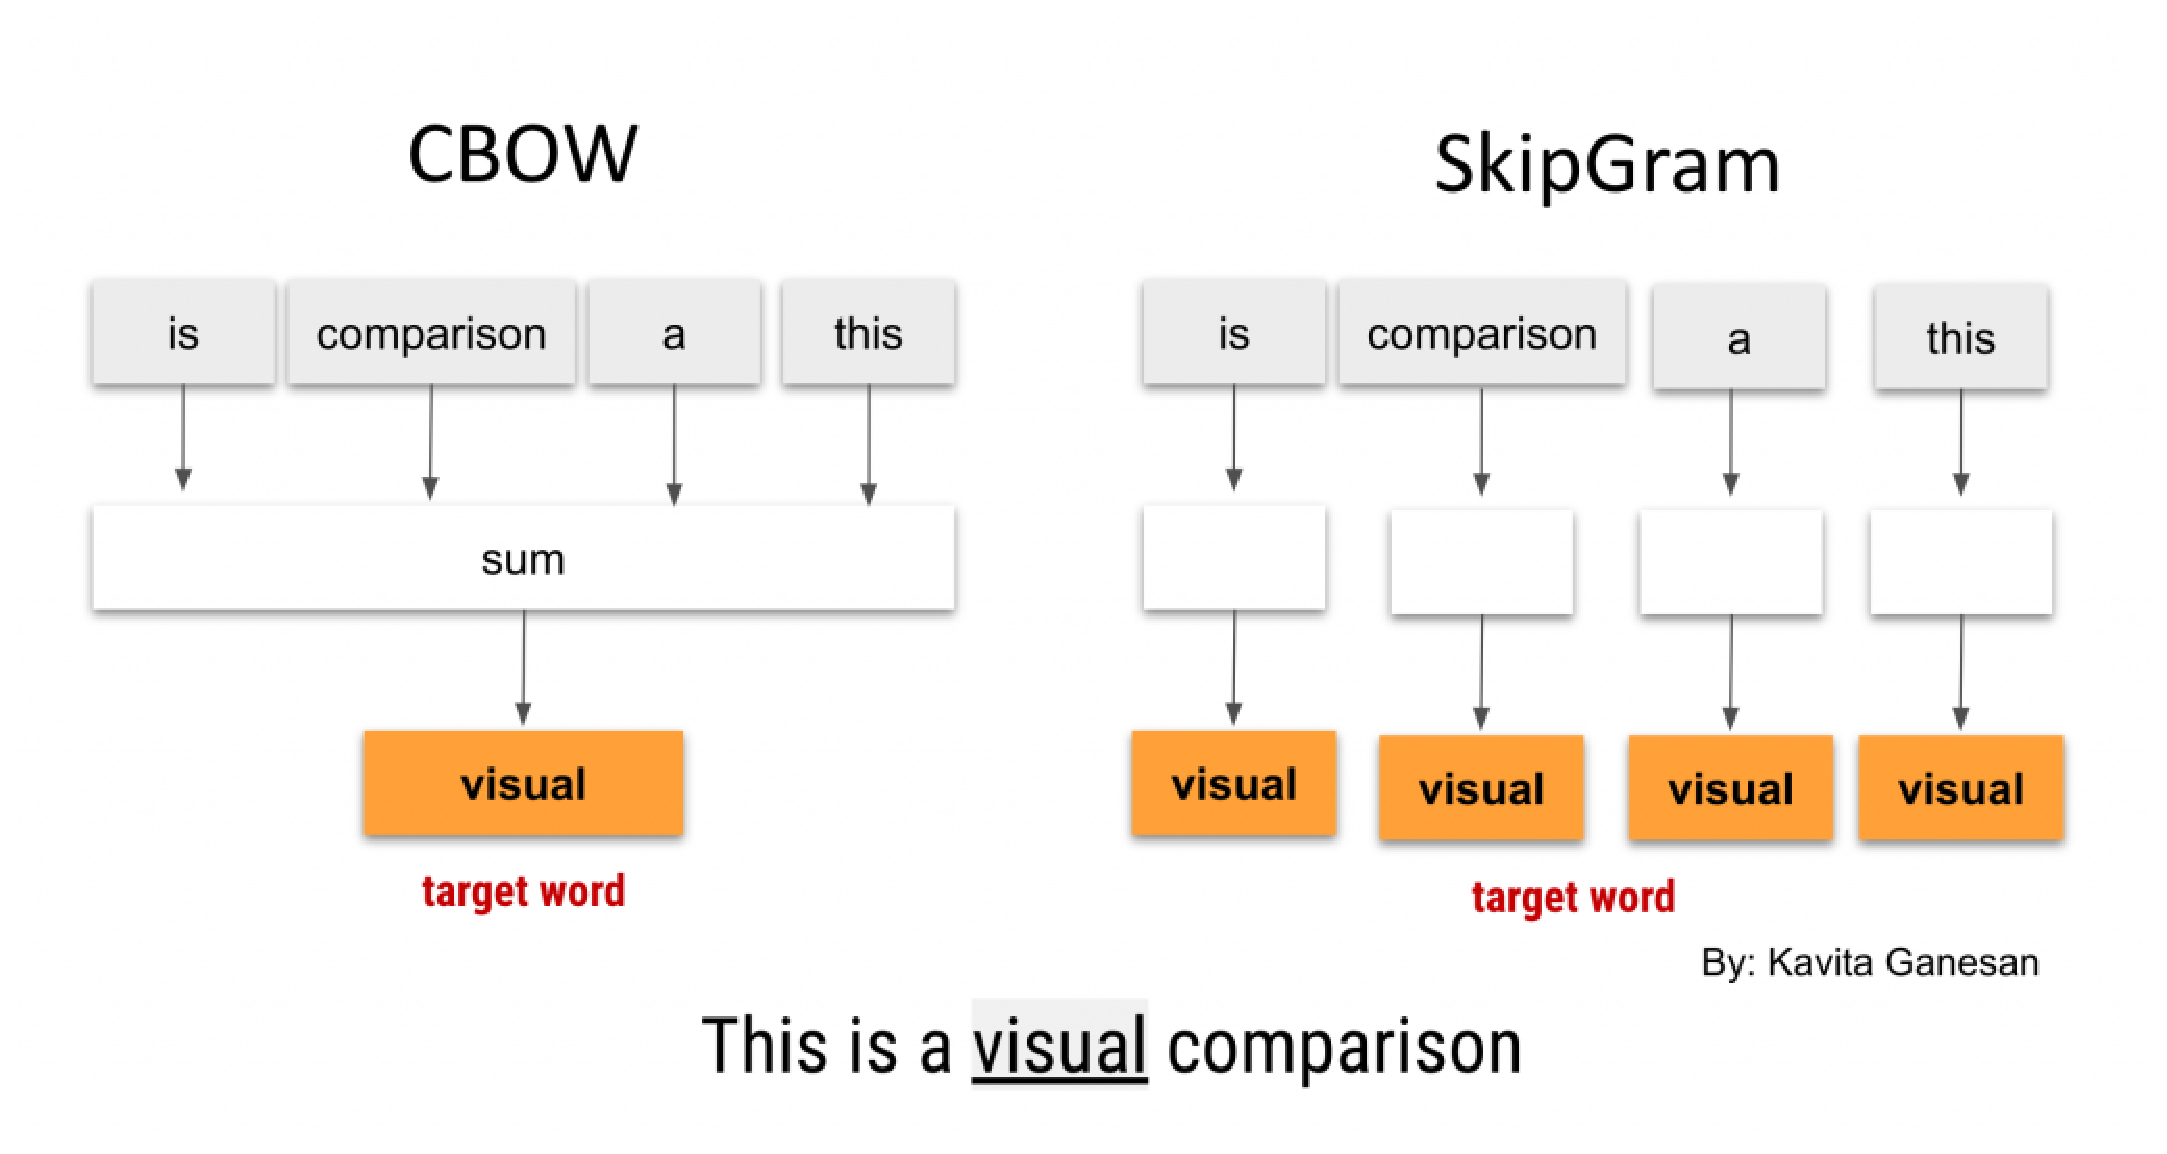
\includegraphics[width=1\textwidth]{figures/skipgram-vs-cbow.eps}
    \footnotesize{(Figure from \href{https://kavita-ganesan.com/comparison-between-cbow-skipgram-subword}{Ganesan, Word2Vec: A Comparison})}
  \end{center}  
\end{slide}

\begin{slide}[toc=Architecture]{Architecture}
  \begin{center}
    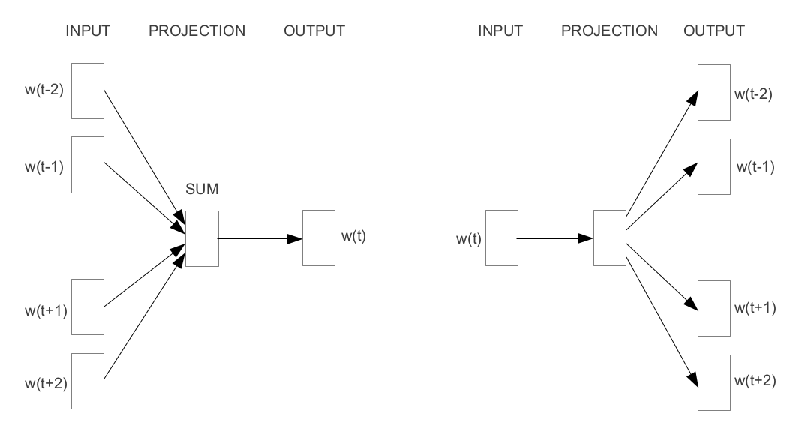
\includegraphics[width=0.8\textwidth]{figures/w2v_arch.eps}
  \end{center}
  While SkipGram simply applies the $E(\cdot)$ embedding mapping to its one-word
  input, CBOW embeds all words in the input skipgram and computes their sum.
  % \parbox{1.1\textwidth}{ \parbox{0.6\textwidth}{
  % text here 
  %   \parbox{{0.4\textwidth}}{
  %     \includegraphics[width=0.4\textwidth]{figures/w2v_cbow.eps}} }
\end{slide}

\begin{slide}[toc=]{Architecture cont.}
  After projecting the input into the word embedding space, both architectures
  use simply a linear projection with weight matrix
  $W \in \mathbb R^{|V|\times d}$ and a final softmax layer to produce
  prediction probabilities for all words in the vocabulary:
   
  \begin{small}
  $$
  CBOW(\langle w_{t-c}\varlist w_{t+c} \rangle) = \softmax(W\sum_{i}E(w_i)),
  $$
  $$
  SkipGram(w_t) = \softmax(W_{}E(w_t)).
  $$
  \end{small}

  Both models are trained with standard negative log likelihood loss and SGD,
  but there are interesting differences regarding the sampling of examples.
\end{slide}

\begin{slide}[toc=]{Architecture cont.}
  It is worth noting that the $W \in \mathbb R^{|V|\times d}$ projection matrix
  can also be seen as an $E'(\cdot)$ embedding of the vocabulary into the same
  $R^d$ space. With this notation, the logits (linear outputs) of the two
  models for a particular $w_j$ word can be written simply as
  \begin{small}
  $$
  CBOW_{linear}(\langle w_{t-c}\varlist w_{t+c} \rangle)[w_j] = E'(w_j)\cdot \sum_{i}E(w_i),
  $$
  $$
  SkipGram_{linear}(w_t)[w_j] = E'(w_j)\cdot E(w_t).
  $$
\end{small}
As this formulation shows, minimizing the negative log likelihood training
objective is a way of increasing the dot product of the embeddings of the input
and that of the correct prediction.
\end{slide}

\begin{slide}[toc=]{Architecture cont.}
  Because of the symmetry shown by this formulation, it is an option to
  \emph{tie the weights} of the two layers making $E(w) = E'(w)$ for all
  $w\in V$.

  Although this is frequently done, it's also customary to keep them different
  and only use the vectors of the input embedding $E(\cdot)$ as the final result, or
  combine them, e.g., by taking their average.
\end{slide}

\begin{slide}[toc=Data generation]{Data point generation and sampling}
  For the CBOW variant, we simply slide the $c$-radius context window through
  the corpus and generate a 
  $$\langle \langle w_{t-c}\varlist w_{t-1}, w_{t+1}\varlist w_{t+c} \rangle, w_t \rangle$$
  $\langle$input, correct output$\rangle$ data point at each step.\bigskip

  The process is more complicated for SkipGram, because at each step the
  actually used context window radius $r$ is randomly chosen from the $[1, c]$
  interval, and a $\langle w_t, w_i\rangle$ data point is generated for each
  $w_i\in \langle w_{t-r}\varlist w_{t-1}, w_{t+1}\varlist w_{t+r}\rangle$ word.
  The effect is that words closer to the target are sampled with a higher
  probability.
\end{slide}

\begin{slide}[toc=Softmax alternatives]{Avoiding full softmax}
  As computing full softmax for a $|V|$-long vector is expensive for large $V$s,
  Word2vec implementations typically use cheaper output layer
  alternatives.\bigskip

  One solution is \emph{\gold hierarchical softmax}, which is based on a binary
  tree whose leaves are the vocabulary words. The linear outputs of the network
  correspond to internal nodes, and the probability assigned to a $w$ word can
  be calculated by computing values of $\sigma(o)$ only for the $o$ outputs that
  lie on the path to $w$. Using a balanced tree this trick reduces the softmax
  computation complexity during training from $\mathcal O(|V|)$ to
  $\mathcal O({\log |V|})$, and with clever tree structure this can be further
  decreased.
\end{slide}

\begin{slide}[toc=]{Hierarchical softmax}
  \begin{center}
    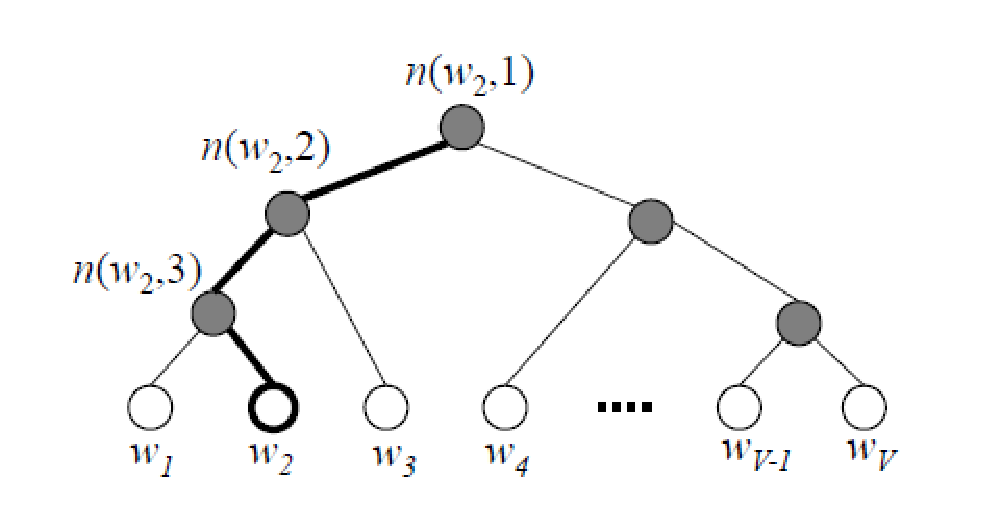
\includegraphics[width=0.65\textwidth]{figures/hierarchic_softmax.eps}
\end{center}
Illustration: if the linear outputs on the path are $o(w_2, 1), o(w_2, 2), o(w_2, 3)$ then the
probability assigned to $w_2$ can be calculated as
$(1-\sigma(o(w_2,1)))(1-\sigma(o(w_2,2)))\sigma(o(w_2,3))=
\sigma(-o(w_2,1))\sigma(-o(w_2,2))\sigma(o(w_2,3))$.
\end{slide}

\begin{slide}[toc=]{Negative sampling}
  The other alternative is \emph{\gold negative
    sampling}\footnote{\citet{mikolov2013distributed}.} This involves
  reformulating the SkipGram task as a binary classification problem.
  \begin{itemize}
  \item We consider earlier SkipGram $\langle$center word, context word$\rangle$
    data points from the corpus as positive examples,
  \item and also generate a certain number of negative examples by sampling, for
    each center word, ``fake context words'' from a noise distribution
    representing the entire corpus.
  \end{itemize}
\end{slide}

\begin{slide}[toc=]{Negative sampling}
  The negative sampling trick makes it possible to simplify the network
  architecture to the point of
  $$
  NSSG(w_{t}, w_{c}) = \sigma(E_t(w_t)\cdot E_c(w_c)) 
  $$
  where $E_t(\cdot)$ is the target (center) word embedding while $E_c(\cdot)$ is
  the context word embedding. With $k$ negative samples from a $P_n$ noise
  distribution, the negative log likelihood loss for each real
  $\langle w_t, w_c\rangle$ data point will be
  $$
  - [ \log NSSG(w_{t}, w_{c}) + \sum_{\substack{i=1 \\ \tilde{w}_i \sim P_n}}^k
  \log(1 - NSSG(w_{t}, {\tilde{w}_i})].  $$
\end{slide}

\begin{slide}[toc=Evaluation]{Evaluation}
  
\end{slide}

\begin{slide}{Bibliography}
  \begin{footnotesize}
    \bibliographystyle{plainnat}
    \bibliography{nlp_course.bib}
  \end{footnotesize}
\end{slide}

\end{document}



%%% Local Variables:
%%% mode: latex 
%%% TeX-master: t
%%% End:

% LocalWords:  Tokenization Discriminative discriminative
